\section{Structure}

The following section describes the essential elements of the overall system in an attempt to make the rest of the report clearer, as we will be describing several components of the system throughout this report.

Being a project that has online capabilities, the \gls{giraf} project has both a backend and some frontend, which in our case, is the Weekplanner application. The communication between these two ends is through a REST \gls{api} and a \gls{fapi}, as illustrated in \autoref{fig:ProductStructure}.

\begin{figure}[H]
    \begin{center}
        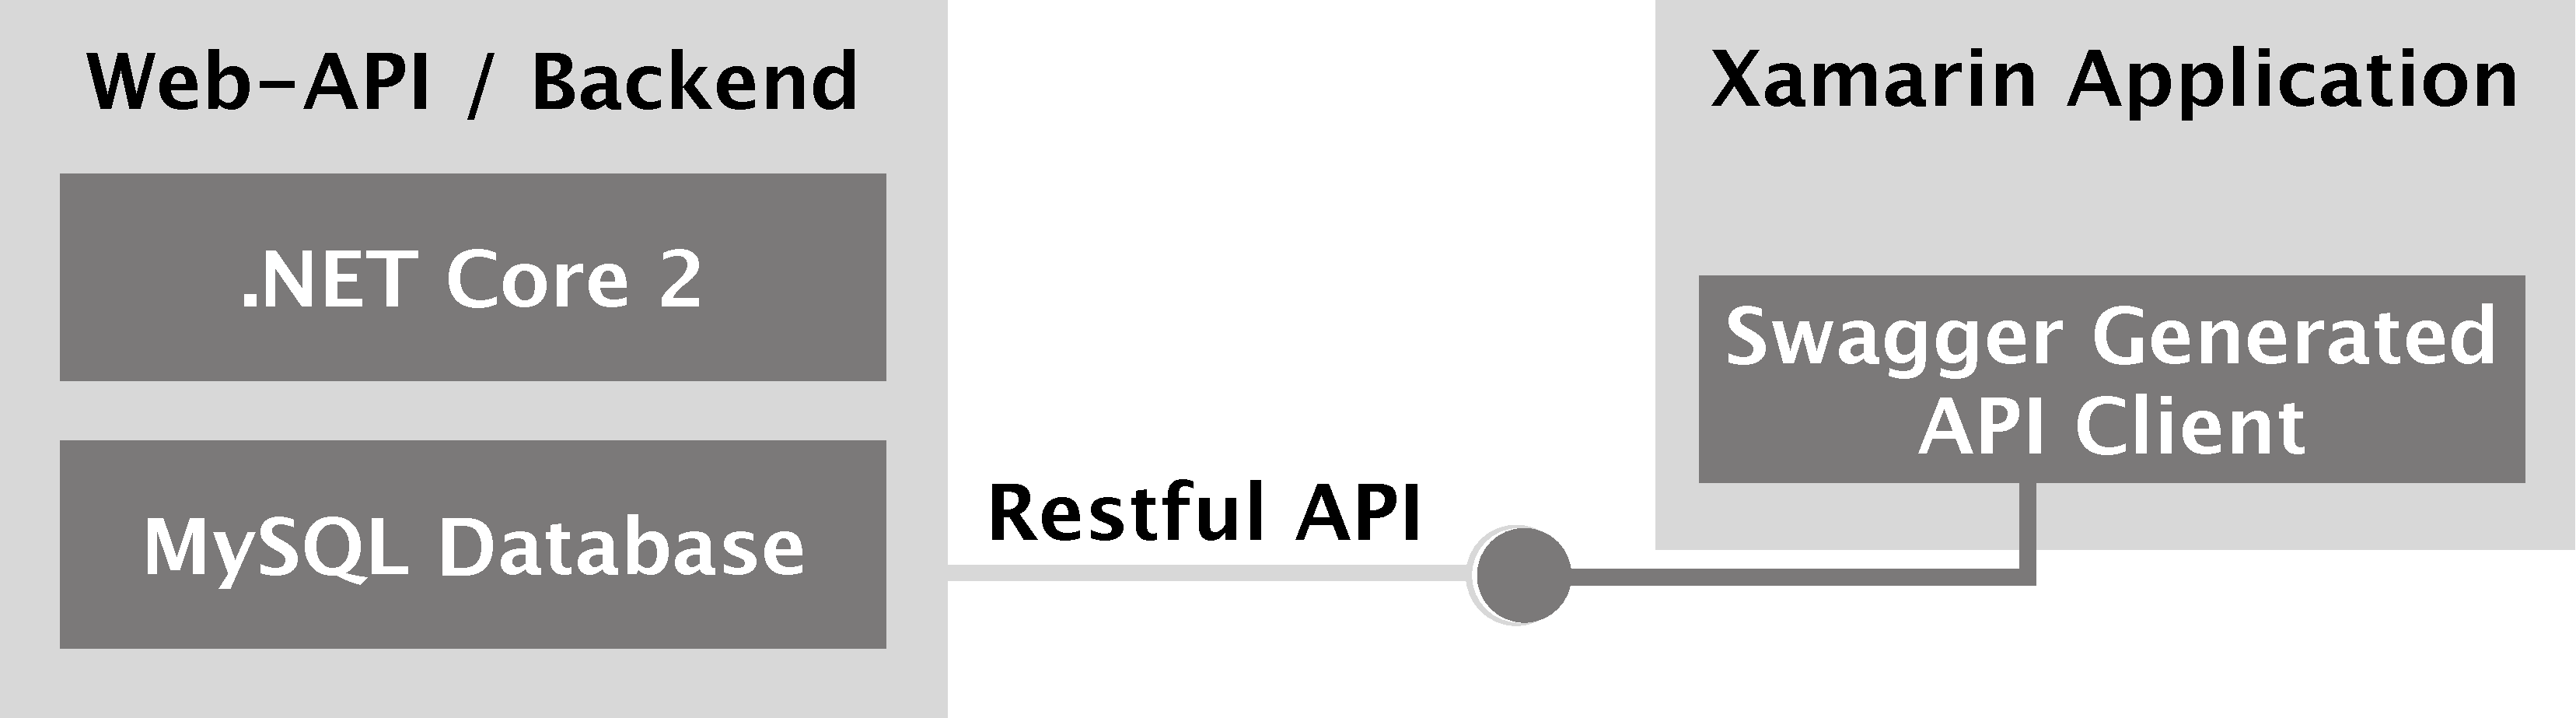
\includegraphics[width=0.95\textwidth]{figures/system_overview.pdf}
    \end{center}
    \caption{The general structure of the \gls{giraf} architecture}
    \label{fig:ProductStructure}
\end{figure}

\subsection{Frontend}

The frontend, built with the Xamarin framework, is the \gls{ui} for the Weekplanner application. The Xamarin framework makes it possible to compile an application for both Android and iOS devices, which enables running the Weekplanner on both of these platforms. The structure of the application is the MVVM pattern (see \cite{davidbritch_model-view-viewmodel} for more information).

\subsection{Server}

The server contains both the database and the backend. The backend is a .NET Core 2 project that uses MVC \cite{ardalis_overview} and supports all the capabilities of the current Weekplanner app.

We can think of the backend as being the bridge between the data stored in the MySQL database and the frontend. As mentioned previously, the frontend can communicate with the backend using the backend's REST \gls{api}.

Being a REST \gls{api} means that the backend should comply with the following principles \cite{REST}:

\begin{itemize}
    \item Separate \gls{ui} and server, which makes scaling easier and the \gls{ui} portable.
    \item The server should be stateless, so all the needed information should be stored in a request rather than as context on the server.
    \item Response data should be cacheable, so a client has the right to store and reuse response data for later requests. 
    \item We should apply the software engineering principle of generality to component interface, which means upholding four interface constraints: identification of resources, manipulation through constraints, self-descriptive messages, and hypermedia as the engine of application state. 
    \item The system should be hierarchically layered, and a component should not be able to see or interact behind the next layer.
    \item (optional) A client should be able to extend functionality with applets or scripts
\end{itemize}

The services hosted on the servers run on an operating-system level virtualization platform called Docker. Docker creates a division between these services by using containers. The goal was to have all of these containers running in a cluster, but at the start of the semester, only some of these containers were. \autoref{fig:state-at-handoff:server} provides a complete overview of the servers and which services they run.

\begin{figure}[h]
    \centering
    \caption{Diagram of the server setup at the time of handoff\cite[p.~74]{SW611F18}}
    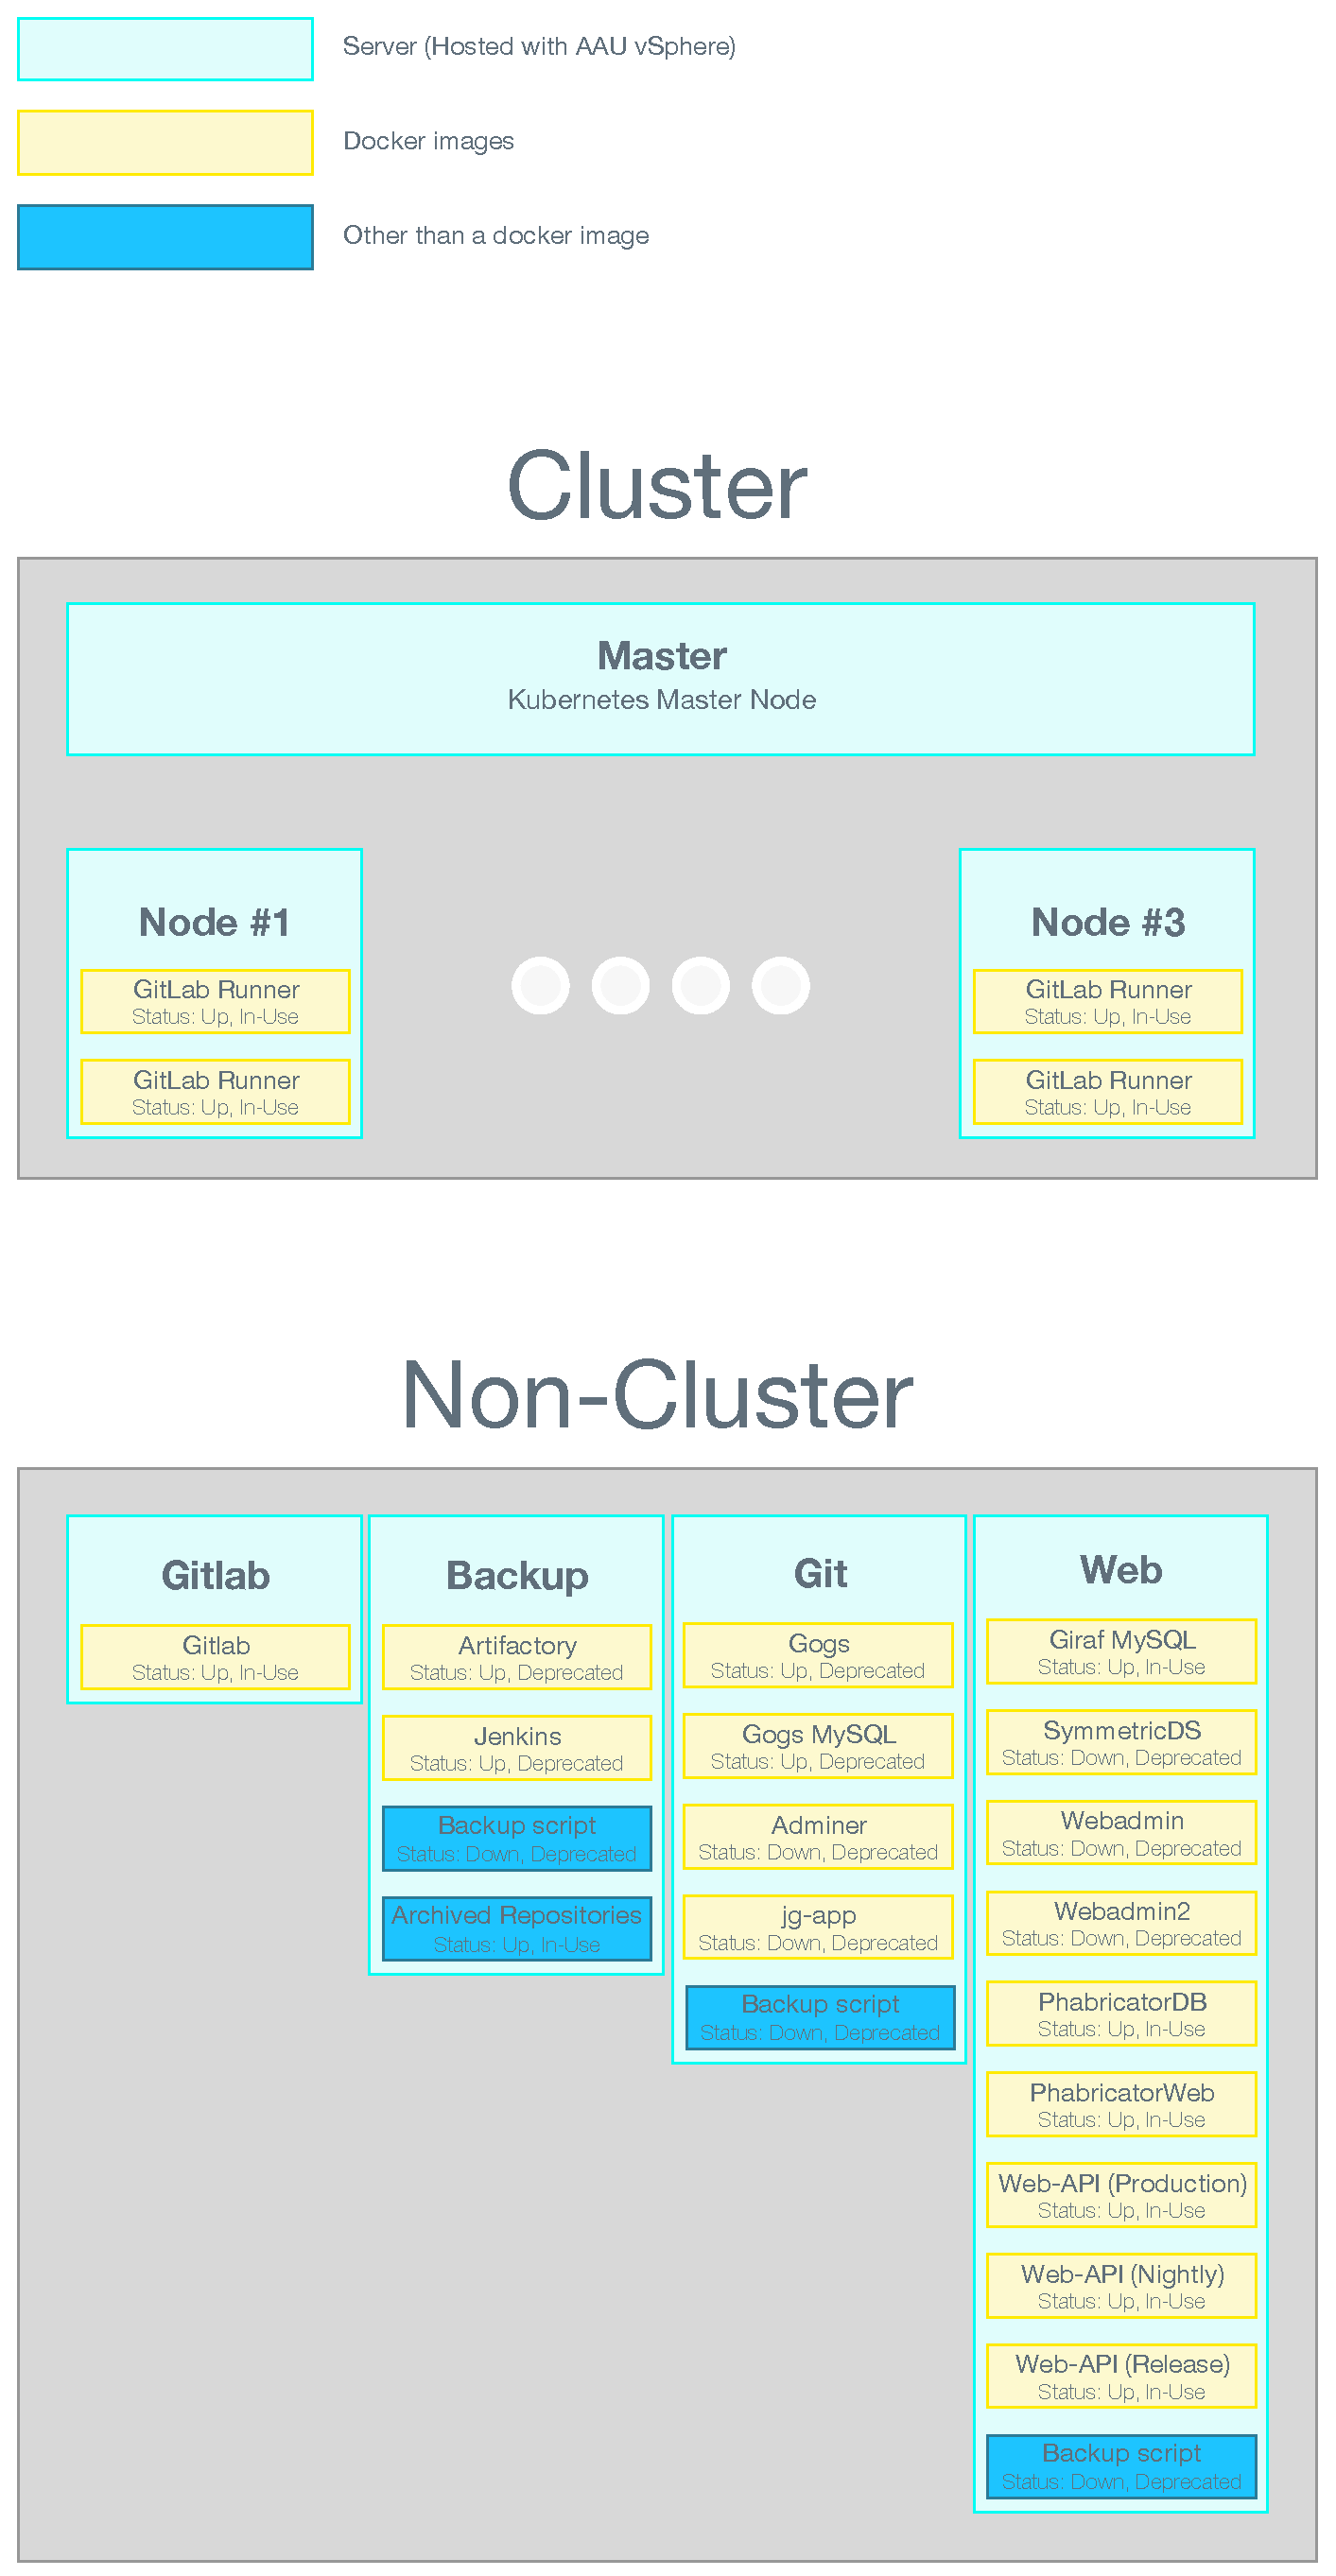
\includegraphics[height=1\textheight]{figures/Server-Overview.pdf}
    \label{fig:state-at-handoff:server}
\end{figure}
